Der Aufbau wird Schritt für Schritt, beginnend an den Detektoren, konfiguriert. 
\subsection{Einstellung des Slow-Koinzidenzkreises}
Zunächst wird das Signal der Dynode vor und nach dem Hauptverstärker auf dem Oszilloskop betrachtet (Abbildung \ref{fig:slow_mit_und_ohne_verstaerkung}). Die Verstärkung ist deutlich zu sehen. Es ist zu sehen, dass die maximale Verstärkung erreicht wird und die stärkeren Pulse somit einem Rechtecksignal ähneln.

\begin{figure}[h]
  \centering
  \begin{tikzpicture}
    \node at (3.25,0) {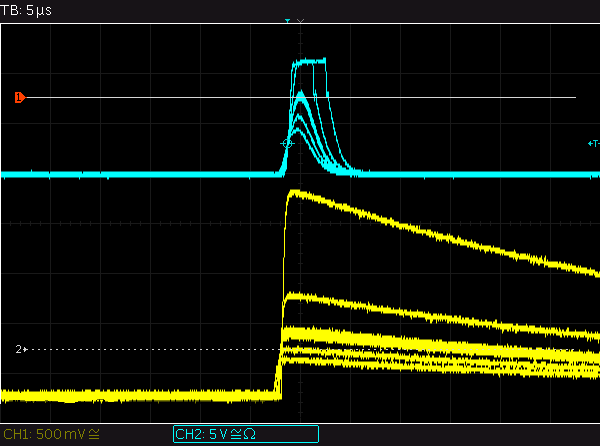
\includegraphics[width=0.45\textwidth]{data/oszi/slow_mit_und_ohne_verstaerkung.png}};
    \draw (-9,-1.25) rectangle (-7,-0.25);
    \draw (-8,-0.5) node {Slow-};
    \draw (-8,-1) node {Ausgang};
    \draw (-7,-0.75)--(-6.5,-0.75)--(-6.5,0.6)--(-6,0.6);
    \draw (-6,0.35)--(-6,0.85)--(-5.5,0.6)--(-6,0.35);
    \draw (-5.5,0.6)--(-0.5,0.6);
    \draw (-6.5,-0.75)--(-6.5,-2.15)--(-0.5,-2.15);
  \end{tikzpicture}
  \caption{Dyodensignal mit und ohne Verstärkung}
  \label{fig:slow_mit_und_ohne_verstaerkung}
\end{figure}
Das Signal des Hauptverstärkers wird mit einem Signalteiler geteilt. Ein Ausgang wird verzögert und einer in den SCA gegeben (bei vollständig geöffnetem Fenster). Die Verstärkung wird so eingestellt, dass die \SI{511}{\kilo\electronvolt} Linie (die das zeitlich stabilste Signal liefert) bei etwa \SI{3.5}{\volt} liegt. Die beiden Signale sind in Abbildung \ref{fig:verstaerkung_auf_3-4v} zu sehen.
\begin{figure}[h]
  \centering
  \begin{tikzpicture}
    \node at (3.25,-0.05) {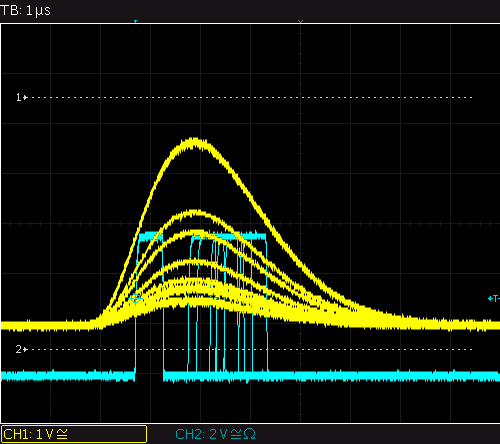
\includegraphics[width=0.45\textwidth]{data/oszi/verstaerkung_auf_3-4v.png}};
    \draw (-9,-1.25-1.6) rectangle (-7,-0.25-1.6);
    \draw (-8,-0.5-1.6) node {Slow-};
    \draw (-8,-1-1.6) node {Ausgang};
    \draw (-7,-0.75-1.6)--(-6.5,-0.75-1.6)--(-6.5,-1-1.6)--(-6,-0.75-1.6)--(-6.5,-0.5-1.6)--(-6.5,-0.75-1.6);
    \draw (-6,-2.35)--(-5.5,-2.35)--(-5.5,-1.6)--(-5,-1.6);
    \draw (-5,-1.35) rectangle (-4,-1.85);
    \draw (-4.5,-1.6) node {Delay};
    \draw (-4,-1.6)--(-0.5,-1.6);
    \draw (-6,-2.35)--(-5,-2.35);
    \draw (-5,-2.1) rectangle (-4,-2.6);
    \draw (-4.5,-2.35) node {SCA};
    \draw (-4,-2.35)--(-0.5,-2.35);
  \end{tikzpicture}
  \caption{Dyodensignal nach Verzögerung bzw. SCA mit angepasster Verstärkung}
  \label{fig:verstaerkung_auf_3-4v}
\end{figure}

Nun wird die Verzögerung so eingestellt, dass beide Signale in etwa synchron sind. Außerdem wird mit dem GDG die Breite des SCA-Pulses so eingestellt, dass das analoge Signal innerhalb des Pulses liegt (Abbildung \ref{fig:zeitliche_breite_sca_und_analog}).
\newpage
\begin{figure}[h]
  \centering
  \begin{tikzpicture}
    \node at (3.25,0) {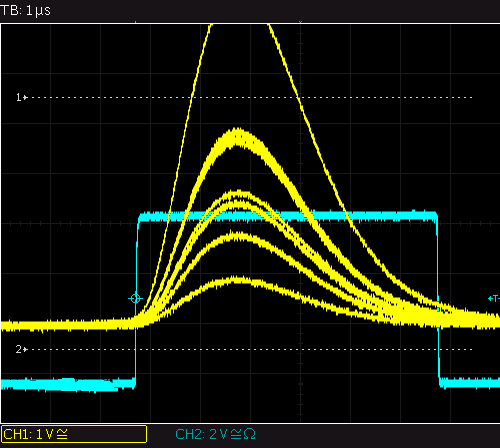
\includegraphics[width=0.45\textwidth]{data/oszi/zeitliche_breite_sca_und_analog.png}};
    \draw (-9,-1.25-1.6) rectangle (-7,-0.25-1.6);
    \draw (-8,-0.5-1.6) node {Slow-};
    \draw (-8,-1-1.6) node {Ausgang};
    \draw (-7,-0.75-1.6)--(-6.5,-0.75-1.6)--(-6.5,-1-1.6)--(-6,-0.75-1.6)--(-6.5,-0.5-1.6)--(-6.5,-0.75-1.6);
    \draw (-6,-2.35)--(-5.5,-2.35)--(-5.5,-1.6)--(-5,-1.6);
    \draw (-5,-1.35) rectangle (-4,-1.85);
    \draw (-4.5,-1.6) node {Delay};
    \draw (-4,-1.6)--(-0.5,-1.6);
    \draw (-6,-2.35)--(-5,-2.35);
    \draw (-5,-2.1) rectangle (-4,-2.6);
    \draw (-4.5,-2.35) node {SCA};
    \draw (-4,-2.35)--(-3.5,-2.35);
    \draw (-3.5,-2.1) rectangle (-2.5,-2.6);
    \draw (-3,-2.35) node {GDG};
    \draw (-2.5,-2.35)--(-0.5,-2.35);
  \end{tikzpicture}
  \caption{Mittels GDG und Verzögerung angepasstes SCA-Signal mit zugehörigem analogen Signal}
  \label{fig:zeitliche_breite_sca_und_analog}
\end{figure}
Die beiden eingestellten Signale dienen nun als Gate-Signal und Eingangssignal des MCA. Bei Aufnahme des Spektrums von $^{22}$Na ist die \SI{511}{\kilo\electronvolt} Linie zu erkennen. Die Verstärkung wird so erhöht, dass die Linie sich am rechten Rand des Spektrums befindet. Anschließend wird das Spektrum von Cs aufgenommen. Die Verstärkung wird so eingestellt, dass die \SI{511}{\kilo\electronvolt} Linie von $^{22}$Na und die \SI{81}{\kilo\electronvolt} Linie von Cs auf dem Spektrum komplett sichtbar sind. Für eine weitere Messung wird das SCA-Fenster so eingestellt, dass nur noch die \SI{511}{\kilo\electronvolt} Linie im Spektrum sichtbar ist. 
\\

Sämtliche bisherigen Schritte werden für den zweiten Detektor wiederholt. Dann werden die SCA-Signale beider Detektoren auf dem Oszilloskop beobachtet und so verzögert, dass sie synchron sind (Abbildung \ref{fig:slow_koinzidenz}).
\begin{figure}[h]
  \centering
  \begin{tikzpicture}
    \node at (3.25,0.05) {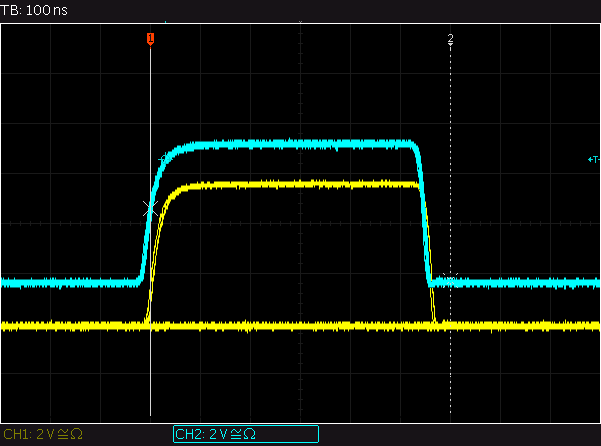
\includegraphics[width=0.45\textwidth]{data/oszi/slow_koinzidenz.png}};
    \draw (-9,-1.25-1.6) rectangle (-7,-0.25-1.6);
    \draw (-8,-0.5-1.6) node {Slow-};
    \draw (-8,-1-1.6) node {Ausgang};
    \draw (-7,-0.75-1.6)--(-6.5,-0.75-1.6)--(-6.5,-1-1.6)--(-6,-0.75-1.6)--(-6.5,-0.5-1.6)--(-6.5,-0.75-1.6);
    \draw (-6,-2.35)--(-5.5,-2.35);
    \draw (-6,-2.35)--(-5,-2.35);
    \draw (-5,-2.1) rectangle (-4,-2.6);
    \draw (-4.5,-2.35) node {SCA};
    \draw (-4,-2.35)--(-2.5,-2.35);
    \draw (-2.5,-2.35)--(-1.9,-2.35);
    \draw (-1.9,-2.35)--(-1.9,-1.25)--(-0.5,-1.25);

    \draw (-9,-1.25-1.6+3.15) rectangle (-7,-0.25-1.6+3.15);
    \draw (-8,-0.5-1.6+3.15) node {Slow-};
    \draw (-8,-1-1.6+3.15) node {Ausgang};
    \draw (-7,-0.75-1.6+3.15)--(-6.5,-0.75-1.6+3.15)--(-6.5,-1-1.6+3.15)--(-6,-0.75-1.6+3.15)--(-6.5,-0.5-1.6+3.15)--(-6.5,-0.75-1.6+3.15);
    \draw (-6,-2.35+3.15)--(-5.5,-2.35+3.15);
    \draw (-6,-2.35+3.15)--(-5,-2.35+3.15);
    \draw (-5,-2.1+3.15) rectangle (-4,-2.6+3.15);
    \draw (-4.5,-2.35+3.15) node {SCA};
    \draw (-4,-2.35+3.15)--(-3.5,-2.35+3.15);
    \draw (-3.5,-2.1+3.15) rectangle (-2.5,-2.6+3.15);
    \draw (-3,-2.35+3.15) node {Delay};
    \draw (-2.5,-2.35+3.15)--(-1.9,-2.35+3.15);
    \draw (-1.9,0.8)--(-1.9,-0.7)--(-0.5,-0.7);
  \end{tikzpicture}
  \caption{Vergleich der zwei SCA-Signale}
  \label{fig:slow_koinzidenz}
\end{figure}

\subsection{Einstellung des Fast-Koinzidenzkreises}
Dyodensignal und Anodensignal werden durch die Betrachtung auf dem Oszilloskop verglichen. Es ist zu sehen, dass das Fast-Signal deutlich schneller ansteigt (Abbildung \ref{fig:slow_fast}). \newpage
\begin{figure}[h]
  \centering
  \begin{subfigure}[h]{0.5\textwidth}
    \centering
    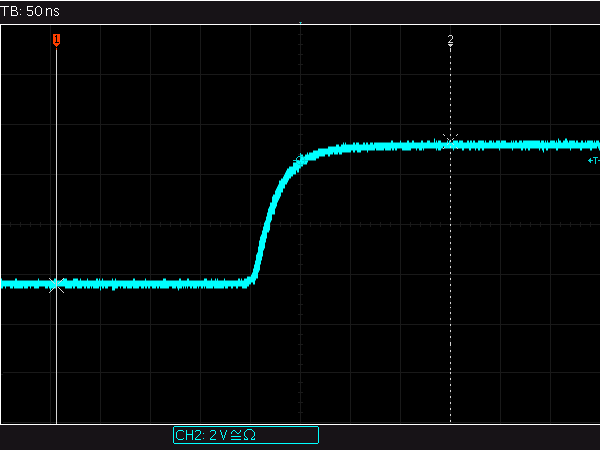
\includegraphics[width=0.9\textwidth]{data/oszi/anstiegszeit_slow.png}
    \subcaption{Anstieg von Slow-Signal}
    \label{fig:anstiegszeit_slow}
  \end{subfigure}%
  \begin{subfigure}[h]{0.5\textwidth}
    \centering
    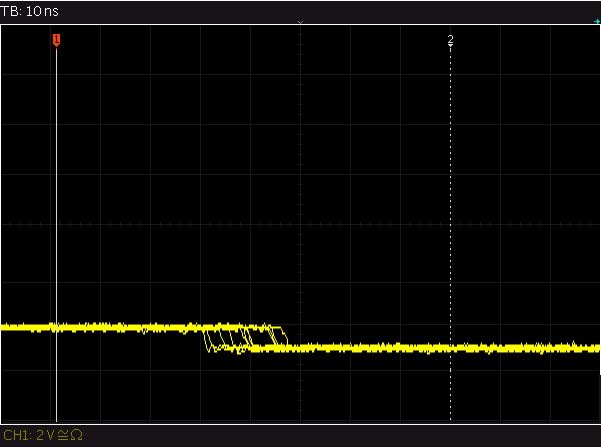
\includegraphics[width=0.9\textwidth]{data/oszi/anstiegszeit_fast.png}
    \subcaption{Anstieg von Fast-Signal}
    \label{fig:anstiegszeit_fast}
  \end{subfigure}
  \caption{Vergleich der Anstiegszeiten von Slow-Signal und Fast-Signal}
  \label{fig:slow_fast}
\end{figure}

Ein Detektor ist sensitiver und sollte somit für die Erzeugung des Stopsignals genutzt werden (Da der zugehörige Übergang Photonen geringerer Energie emittiert). Anhand des Vergleiches der beiden Anodensignale in Abbildung \ref{fig:detektorvergleich} kann der bessere Detektor (mit höherer Signalamplitude) bestimmt werden.
\begin{figure}[h]
  \centering
  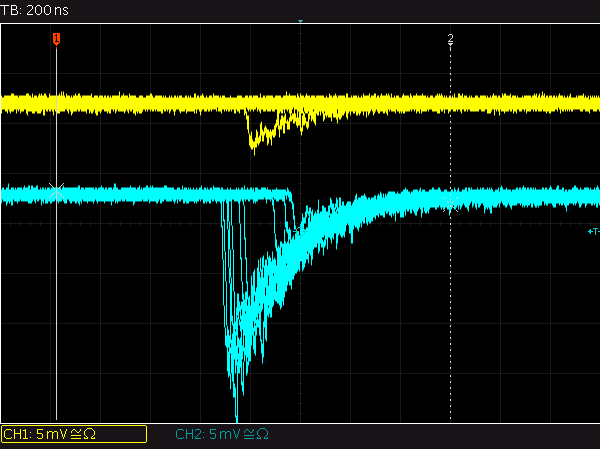
\includegraphics[width=0.5\textwidth]{data/oszi/detektorvergleich.png}
  \caption{Vergleich der Anodensignale beider Detektoren}
  \label{fig:detektorvergleich}
\end{figure}

Start- und Stop-Signal werden zeitlich so verzögert, dass das Stop-Signal etwa \SI{150}{\nano\second} nach dem Start-Signal kommt (Abbildung \ref{fig:zeitabstand_fast}). 
\newpage
\begin{figure}[h]
  \centering
  \begin{tikzpicture}
    \node at (3.25,0.1) {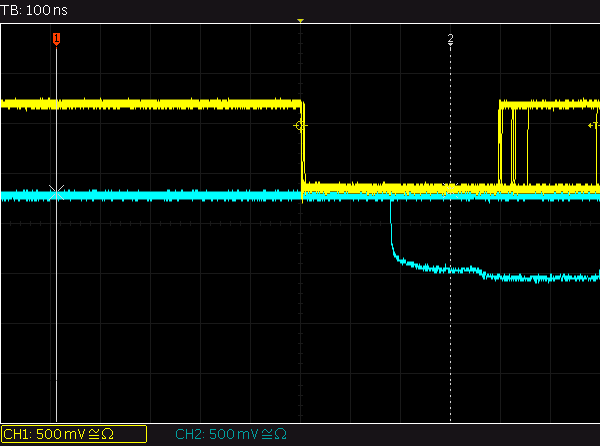
\includegraphics[width=0.45\textwidth]{data/oszi/zeitabstand_fast.png}};
    \draw (-9,-1.25-1.6+3.95) rectangle (-7,-0.25-1.6+3.95);
    \draw (-8,-0.5-1.6+3.95) node {Fast-};
    \draw (-8,-1-1.6+3.95) node {Ausgang};
    \draw (-7,-0.75-1.6+3.95)--(-6,-0.75-1.6+3.95);
    \draw (-6,-2.35+3.95)--(-5.5,-2.35+3.95);
    \draw (-6,-2.35+3.95)--(-5,-2.35+3.95);
    \draw (-5,-2.1+3.95) rectangle (-4,-2.6+3.95);
    \draw (-4.5,-2.35+3.95) node {CFD};
    \draw (-4,-2.35+3.95)--(-2.5,-2.35+3.95);
    \draw (-2.5,-2.35+3.95)--(-0.5,-2.35+3.95);
    
    \draw (-9,-1.25-1.6+2.8) rectangle (-7,-0.25-1.6+2.8);
    \draw (-8,-0.5-1.6+2.8) node {Fast-};
    \draw (-8,-1-1.6+2.8) node {Ausgang};
    \draw (-7,-0.75-1.6+2.8)--(-6,-0.75-1.6+2.8);
    \draw (-6,-2.35+2.8)--(-5.5,-2.35+2.8);
    \draw (-6,-2.35+2.8)--(-5,-2.35+2.8);
    \draw (-5,-2.1+2.8) rectangle (-4,-2.6+2.8);
    \draw (-4.5,-2.35+2.8) node {CFD};
    \draw (-4,-2.35+2.8)--(-3.5,-2.35+2.8);
    \draw (-3.5,-2.1+2.8) rectangle (-2.5,-2.6+2.8);
    \draw (-3,-2.35+2.8) node {Delay};
    \draw (-2.5,-2.35+2.8)--(-0.5,-2.35+2.8);
  \end{tikzpicture}
  \caption{Zeitliche Lage von Start- und Stop-Signal}
  \label{fig:zeitabstand_fast}
\end{figure}

Nun muss noch die zeitliche Koinzidenz von den beiden Kreisen eingestellt werden. Dazu werden das Koinzidenzsignal vom Slow-Kreis und das SIgnal des TAC auf dem Oszilloskop beobachtet. Mit Hilfe des GDG werden die Signale synchronisiert (Abbildung \ref{fig:fast_und_slow}).
\begin{figure}[h]
  \centering
  \begin{tikzpicture}
    \node at (3.25,0) {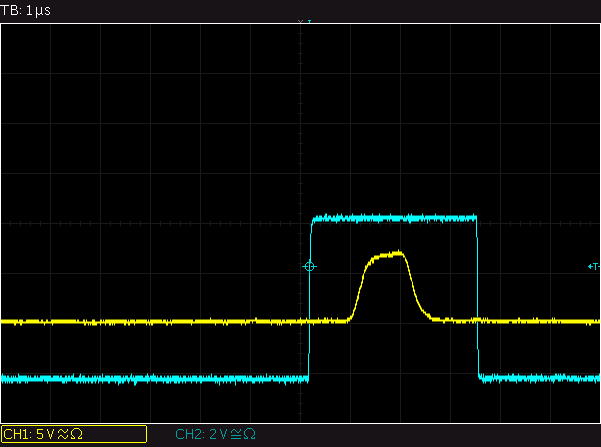
\includegraphics[width=0.45\textwidth]{data/oszi/fast_und_slow.png}};
    \draw (-9,-1.25-1.6+3.95) rectangle (-7,-0.25-1.6+3.95);
    \draw (-8,-0.5-1.6+3.95) node {Fast-};
    \draw (-8,-1-1.6+3.95) node {Ausgang};
    \draw (-7,-0.75-1.6+3.95)--(-1-5,-0.75-1.6+3.95);
    \draw (-1-5,-2.1+3.95) rectangle (-1-4,-2.6+3.95);
    \draw (-1-4.5,-2.35+3.95) node {CFD};
    \draw (-1-4,-2.35+3.95)--(-1-1.4+0.5,-2.35+3.95)--(-1.9,0);
    \draw (-9,-1.25-1.6+2.8) rectangle (-7,-0.25-1.6+2.8);
    \draw (-8,-0.5-1.6+2.8) node {Fast-};
    \draw (-8,-1-1.6+2.8) node {Ausgang};
    \draw (-7,-0.75-1.6+2.8)--(-1-5,-0.75-1.6+2.8);
    \draw (-1-5,-2.1+2.8) rectangle (-1-4,-2.6+2.8);
    \draw (-1-4.5,-2.35+2.8) node {CFD};
    \draw (-1-4,-2.35+2.8)--(-1-3.5,-2.35+2.8);
    \draw (-1-3.5,-2.1+2.8) rectangle (-1-2.5,-2.6+2.8);
    \draw (-1-3,-2.35+2.8) node {Delay};
    \draw (-1-2.5,-2.35+2.8)--(-1-1.4,-2.35+2.8)--(-2.4,0);
    \draw (-2.65,0) rectangle (-1.65,-0.5);
    \draw (-2.15,-0.25) node {TAC};
    \draw (-2.15,-0.5)--(-2.15,-1.2)--(-0.5,-1.2);

    \draw (-9,-1.25-1.6+3.95-2.525-0.45) rectangle (-7,-0.25-1.6+3.95-2.525-0.45);
    \draw (-8,-0.5-1.6+3.95-2.525-0.45) node {Slow-};
    \draw (-8,-1-1.6+3.95-2.525-0.45) node {Ausgang};
    \draw (-7,-0.75-1.6+3.95-2.525-0.45)--(-6.75,-0.925-0.45)--(-6.75,-1.175-0.45)--(-6.25,-0.925-0.45)--(-6.75,-0.675-0.45)--(-6.75,-0.925-0.45);
    \draw (-6.25,-0.925-0.45)--(-1-5,-0.75-1.6+3.95-2.525-0.45);
    \draw (-1-5,-2.1+3.95-2.525-0.45) rectangle (-1-4,-2.6+3.95-2.525-0.45);
    \draw (-1-4.5,-2.35+3.95-2.525-0.45) node {SCA};
    \draw (-1-4,-2.35+3.95-2.525-0.45)--(-3.25,-2.35+3.95-2.525-0.45)--(-3.25,-1.4-0.45)--(-3,-1.4-0.45);
    \draw (-9,-1.25-1.6+2.8-2.525-0.45) rectangle (-7,-0.25-1.6+2.8-2.525-0.45);
    \draw (-8,-0.5-1.6+2.8-2.525-0.45) node {Slow-};
    \draw (-8,-1-1.6+2.8-2.525-0.45) node {Ausgang};
    \draw (-7,-0.75-1.6+2.8-2.525-0.45)--(-6.75,-0.925-1.15-0.45)--(-6.75,-1.175-1.15-0.45)--(-6.25,-0.925-1.15-0.45)--(-6.75,-0.675-1.15-0.45)--(-6.75,-0.925-1.15-0.45);
    \draw (-6.25,-0.925-1.15-0.45)--(-1-5,-0.75-1.6+2.8-2.525-0.45);
    \draw (-1-5,-2.1+2.8-2.525-0.45) rectangle (-1-4,-2.6+2.8-2.525-0.45);
    \draw (-1-4.5,-2.35+2.8-2.525-0.45) node {SCA};
    \draw (-1-4,-2.35+2.8-2.525-0.45)--(-1-3.5,-2.35+2.8-2.525-0.45);
    \draw (-1-3.5,-2.1+2.8-2.525-0.45) rectangle (-1-2.5,-2.6+2.8-2.525-0.45);
    \draw (-1-3,-2.35+2.8-2.525-0.45) node {Delay};
    \draw (-1-2.5,-2.35+2.8-2.525-0.45)--(-3.25,-2.35+2.8-2.525-0.45)--(-3.25,-1.6-0.45)--(-3,-1.6-0.45);
    \draw (-3,-1.75-0.45) rectangle (-2,-1.25-0.45);
    \draw (-2.5,-1.5-0.45) node {Coinc.};
    \draw (-2,-1.5-0.45)--(-1.75,-1.5-0.45);
    \draw (-1.75,-1.75-0.45) rectangle (-0.75,-1.25-0.45);
    \draw (-1.25,-1.5-0.45) node {GDG};
    \draw (-0.75,-1.95)--(-0.5,-1.95);
  \end{tikzpicture}
  \caption{TAC-Signal aus Fast-Kreis und Gate-Signal aus Slow-Kreis}
  \label{fig:fast_und_slow}
\end{figure}

\subsection{Zeitkalibration}
Für die Auswertung muss der funktionale Zusammenhang von dem TAC-Signal (bzw. dem dazugehörigen Bin des MCA) und der entsprechenden Zeit bestimmt werden. Dazu wird mit dem MCA das (zeitliche) Spektrum der \SI{511}{\kilo\electronvolt} Linie aufgenommen. Durch das schrittweise Zuschalten einer \SI{16}{\nano\second} Verzögerung entstehen sieben Promptkurven im Spektrum deren Abstand jeweils \SI{16}{\nano\second} entspricht. 

\subsection{Lebensdauermessung}
Erneut werden mit dem MCA die Spektren von $^{22}$Na und Cs aufgenommen. Das SCA-Fenster der Detektoren wird nun für den besseren (schlechteren) Detektor auf die relevante bevölkernde (entvölkernde) Linie von Cs eingestellt. Nach erneuter Überprüfung der Koinzidenz der beiden Messkreise auf dem Oszilloskop kann die eigentliche Lebensdauermessung gestartet werden. 
